
\vspace{1.5cm}


Para lograr la conmutación de la carga se utilizó el circuito mostrado en la figura~\figref{fig:fig_p16_rl_switch}, donde se puede ver el modelo de una llave controlada por tensión con resistencia de $0 \si[per-mode=symbol]{\ohm}$ en estado cerrado y resistencia tendiendo a infinito (valor muy grande) para el estado abierto. El switch es controlado por una onda cuadrada, de tal manera de lograr una carga de $0 \si[per-mode=symbol]{\ampere}$ al comienzo de la simulación, de $1 \si[per-mode=symbol]{\ampere}$ ($R_{L} = 2 \si[per-mode=symbol]{\ohm}$) a los $20 \si[per-mode=symbol]{\milli\second}$, y luego nuevamente $0 \si[per-mode=symbol]{\ampere}$ a los $50 \si[per-mode=symbol]{\milli\second}$. La simulación realizada es del tipo transitorio (\textbf{SPICE} \textit{.tran}), la salida de la misma se muestra resaltando el momento de las transiciones en la figura~\figref{fig:fig_p16_output_in_load_jump}. En la figura~\figref{fig:fig_p16_output_variation_in_load_jump} se destaca la diferencia en la tensión de salida en carga respecto a en vacío, esta diferencia permite estimar la resistencia de salida de la fuente de alimentación, el valor obtenido es:\\


\begin{equation}
R_{o} = \frac{\Delta V}{\Delta I} = \frac{\num{3.67E-4} \si[per-mode=symbol]{\volt}}{1.0137 \si[per-mode=symbol]{\ampere}} = 642 \si[per-mode=symbol]{\micro\ohm}
\end{equation}

\begin{figure}[H] %htb
\begin{center}
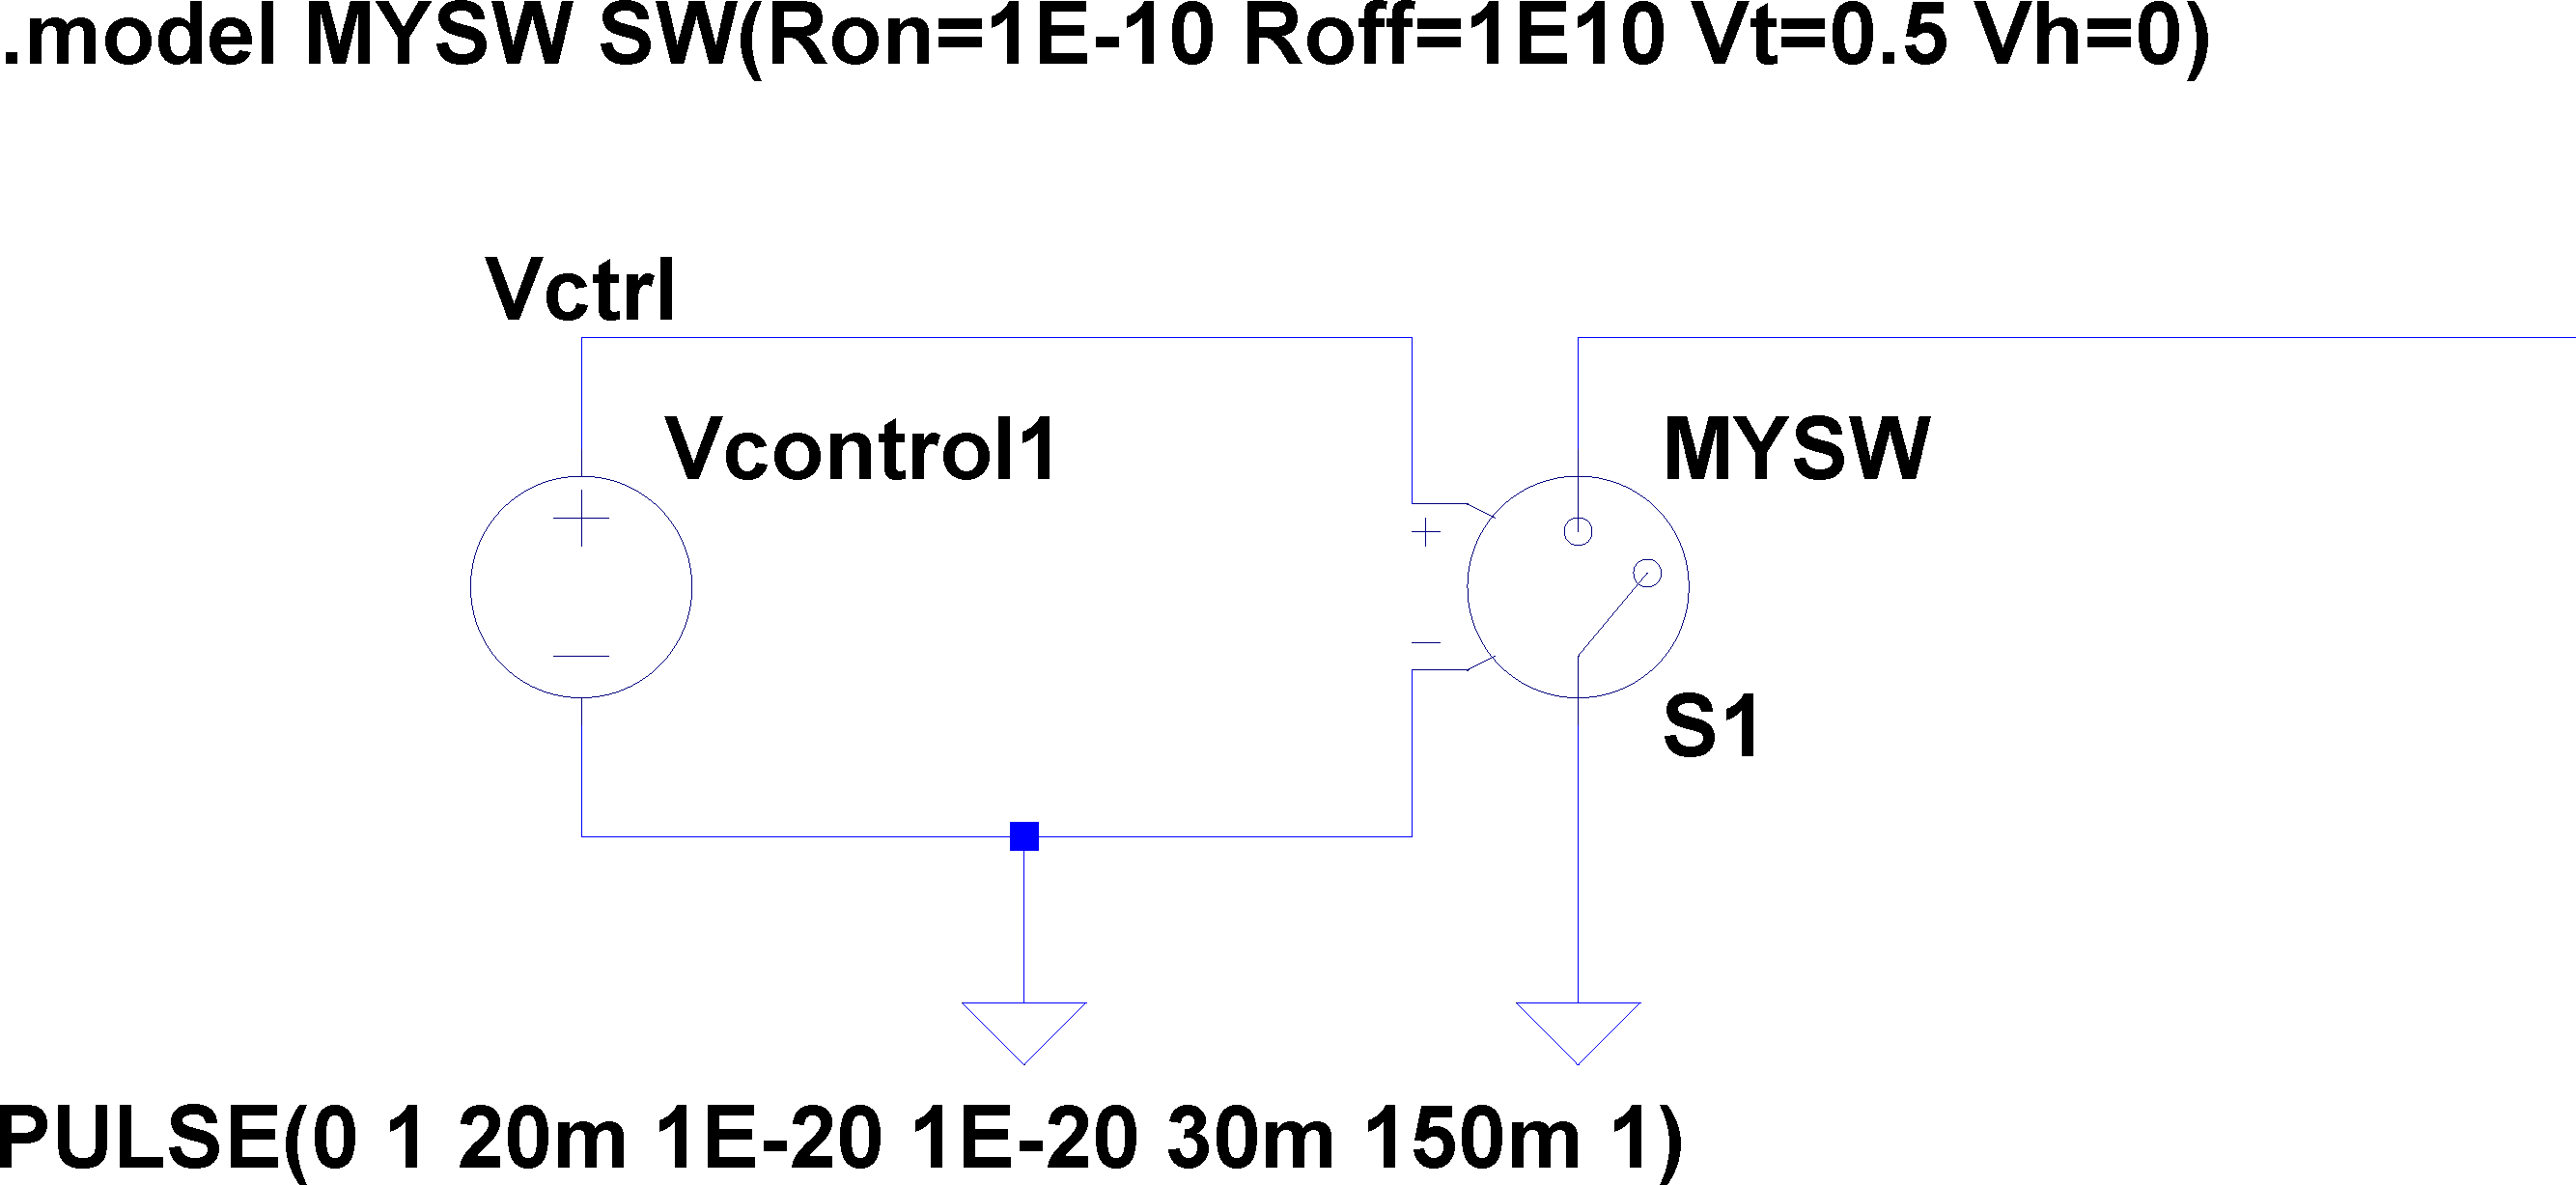
\includegraphics[width=0.9 \textwidth, angle=0]{./img/preguntas/p16a.png}
\caption{\label{fig:fig_p16_rl_switch}\footnotesize{Circuito usado para la conmutación de la carga}}
\end{center}
\end{figure}


\vfill

\clearpage

\begin{figure}[H] %htb
\begin{center}
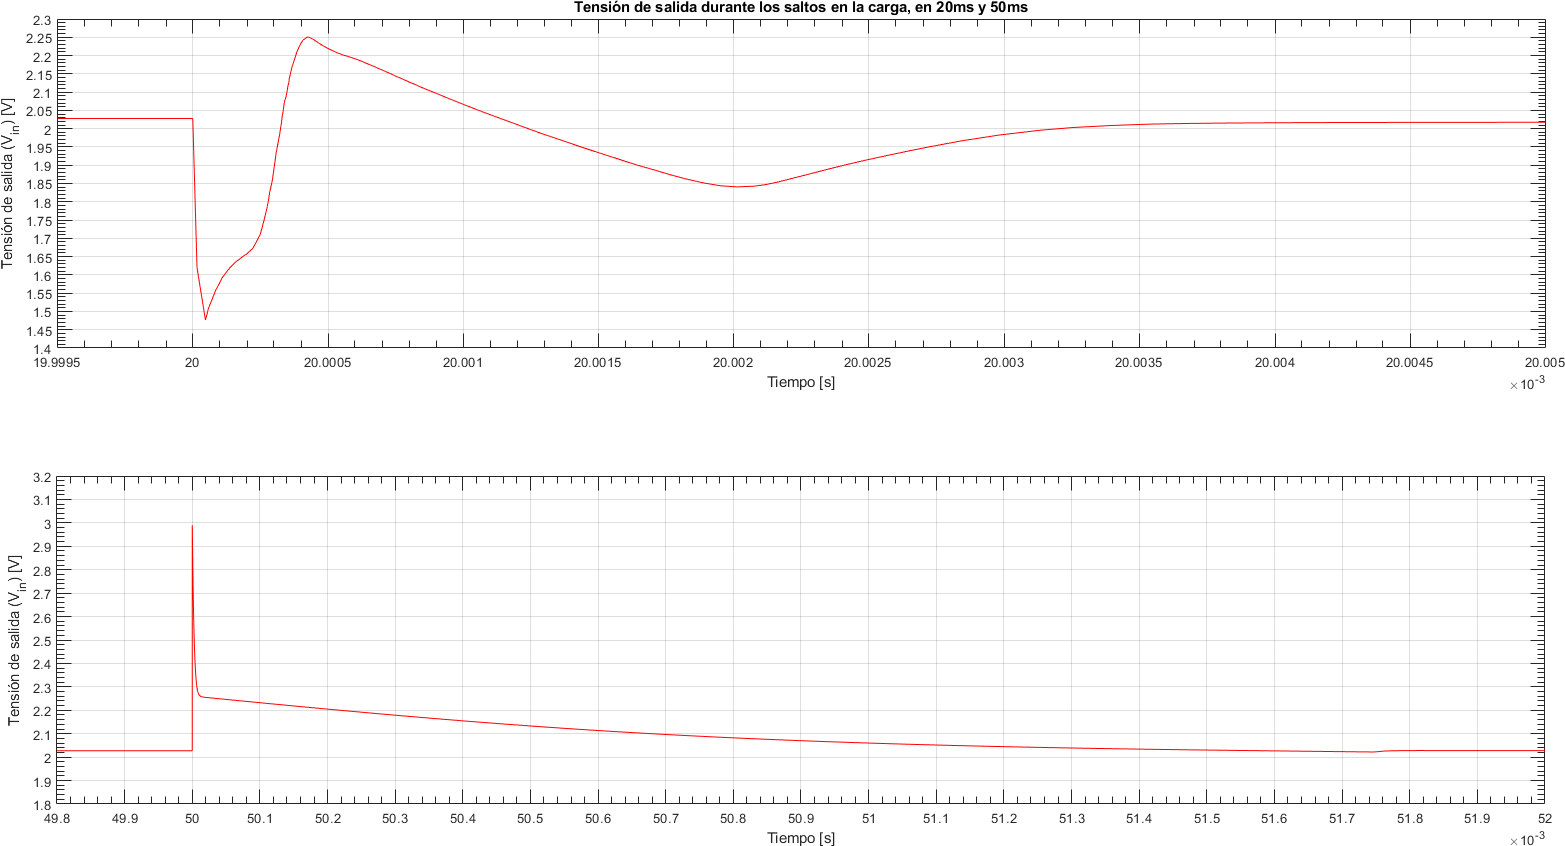
\includegraphics[width=1.2 \textwidth, angle=90]{./img/preguntas/p16b.png}
\caption{\label{fig:fig_p16_output_in_load_jump}\footnotesize{Tensión de salida frente a saltos de carga de $0 \si[per-mode=symbol]{\ampere}$ a $1 \si[per-mode=symbol]{\ampere}$ y de $1 \si[per-mode=symbol]{\ampere}$ a $0 \si[per-mode=symbol]{\ampere}$.}}
\end{center}
\end{figure}


\clearpage

\begin{figure}[H] %htb
\begin{center}
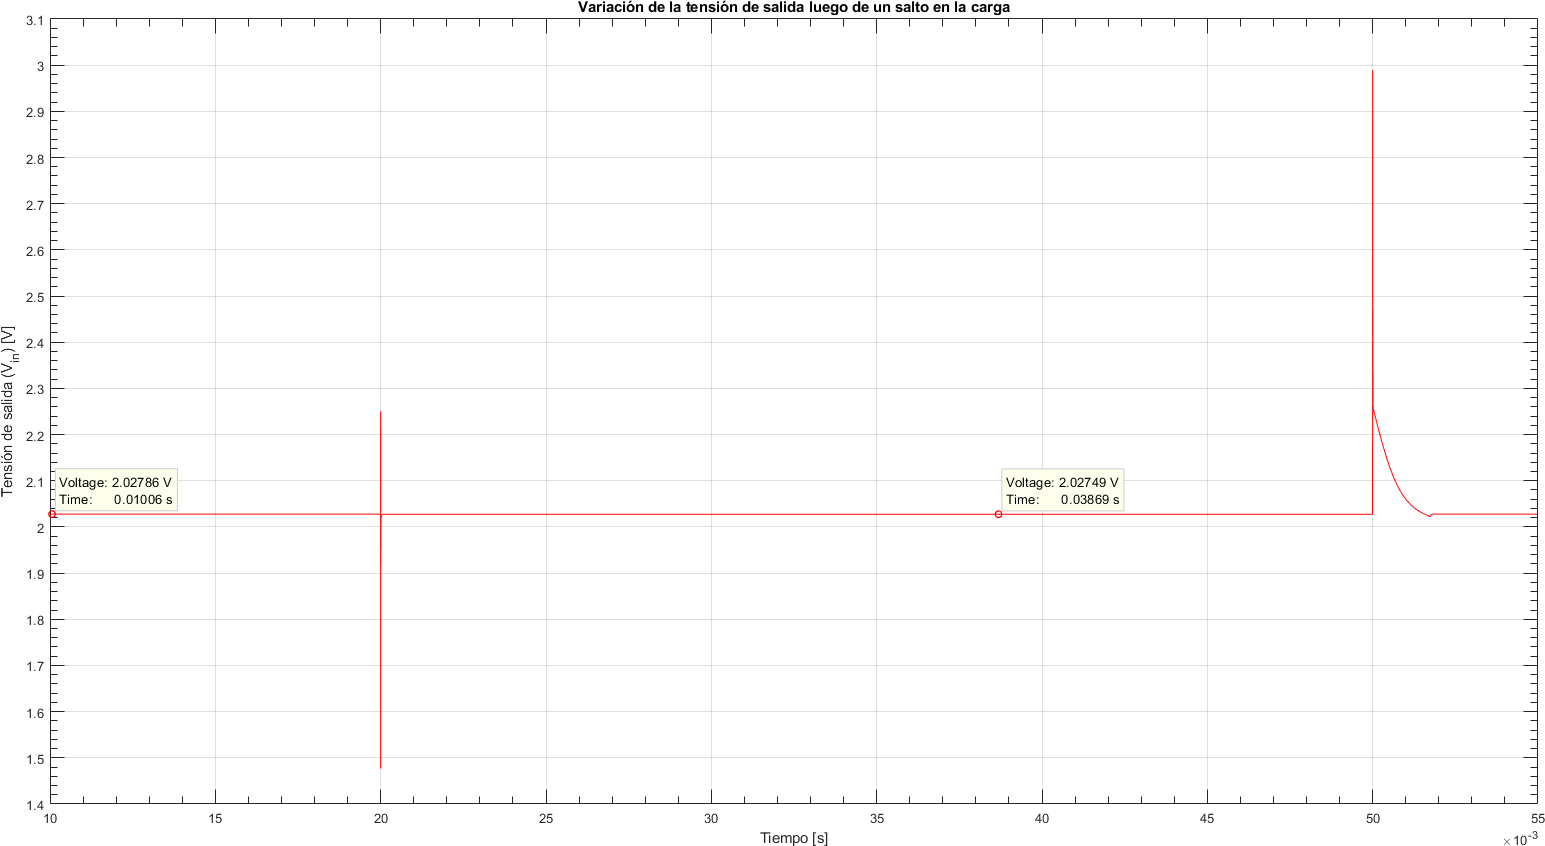
\includegraphics[width=1.2 \textwidth, angle=90]{./img/preguntas/p16c.png}
\caption{\label{fig:fig_p16_output_variation_in_load_jump}\footnotesize{Variación de la tensión de salida en los saltos de carga}}
\end{center}
\end{figure}




\clearpage
